\section{ソフトウェア最適化}
本コンテストでは 1216*1936 の車載カメラ画像の Semantic Segmentation を行うことが課題として設定されている.
具体的には,入力画像の各ピクセルに対して4カテゴリ (乗用車,歩行者,信号,車道・駐車場)
の分類を行った結果を出力する推論アプリケーションの実装が求められる.

我々の実装では,
入力画像の縮小 (1216*1936 $\rightarrow$ 320*640) ,および,正規化を行った後にDPUによる推論を行う.
また,DPUによる推論の結果は,ラベル付け,および,入力画像と同サイズへの拡大 (320*640 $\rightarrow$ 1216*1936) を行うことで出力画像となる.
ところで,本コンテストのルールでは,入力画像のメモリ上へのロード,および,出力画像のファイル出力は推論処理時間に含めない.
よって,上記の前処理(縮小・正規化),推論(DPU実行),後処理(ラベル付け・拡大)の3つの処理が推論処理時間計測の対象となる.

我々はこれらの処理のマルチスレッド実装を行った.
DPUによる推論の実行中に,次の画像の前処理,および,前の画像の後処理を行うことで,
シーケンシャルに処理する場合に比べて大幅な高速化が見込まれる.

本章では,はじめに上記の処理をシングルスレッド実装する場合についての説明を行う.
その後,マルチスレッド実装についての説明を行う.

\subsection{シングルスレッド実装}
図 \ref{fig:singlethread} に我々の推論処理をシングルスレッドで実装する場合のフローチャートを示す.

\begin{figure}[h]
  \begin{center}
    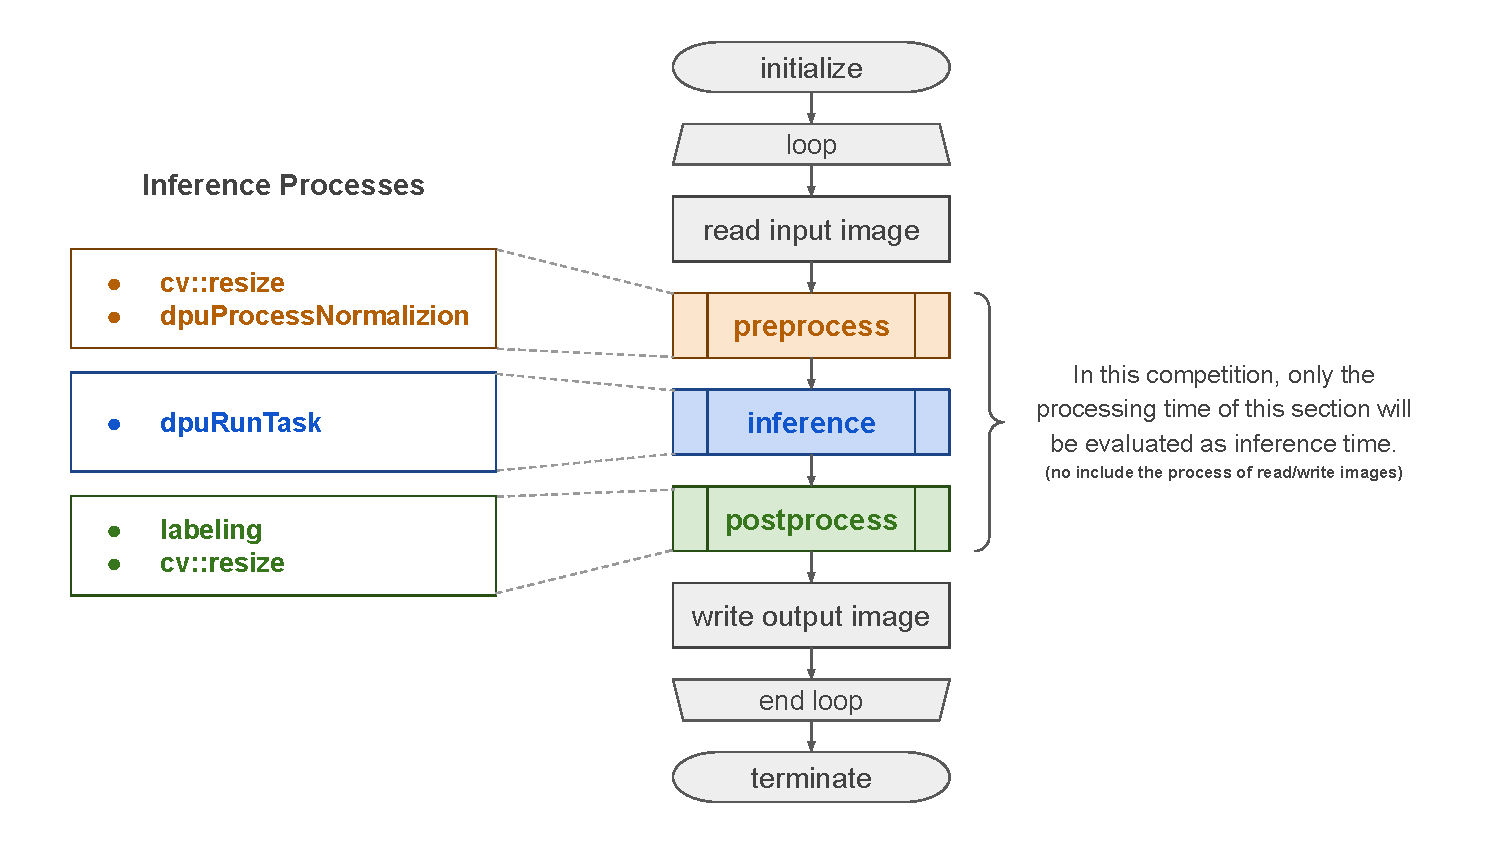
\includegraphics[width=\linewidth]{figures/sw_opt_flowchart_singlethread.pdf}
    \caption{シングルスレッド実行時}
    \label{fig:singlethread}
  \end{center}
\end{figure}

シングルスレッド実装を行う場合,
画像を1枚読み込み,推論を行い,推論結果を書き込む処理をテスト画像全てに対して繰り返す実装が考えられる.
前処理(preprocess),推論処理(inference),後処理(postprocess)の実行区間が推論処理時間計測の対象である.
前処理では,OpenCVの関数cv::resizeを用いて入力画像の縮小を行い,
Vitis-AIのDPUライブラリの関数dpuProcessNormalizionによって各画素値の正規化を行う.
推論処理では,DPUによる推論を行う関数dpuRunTaskを実行する.
後処理では,推論結果を参照してラベル画像を生成し,
その後,関数cv::resizeを用いてラベル画像の拡大を行う.

\subsection{マルチスレッド実装}
今回我々が実装したマルチスレッド実装の概要を図 \ref{fig:multithread} に示す.

\begin{figure}[h]
  \begin{center}
    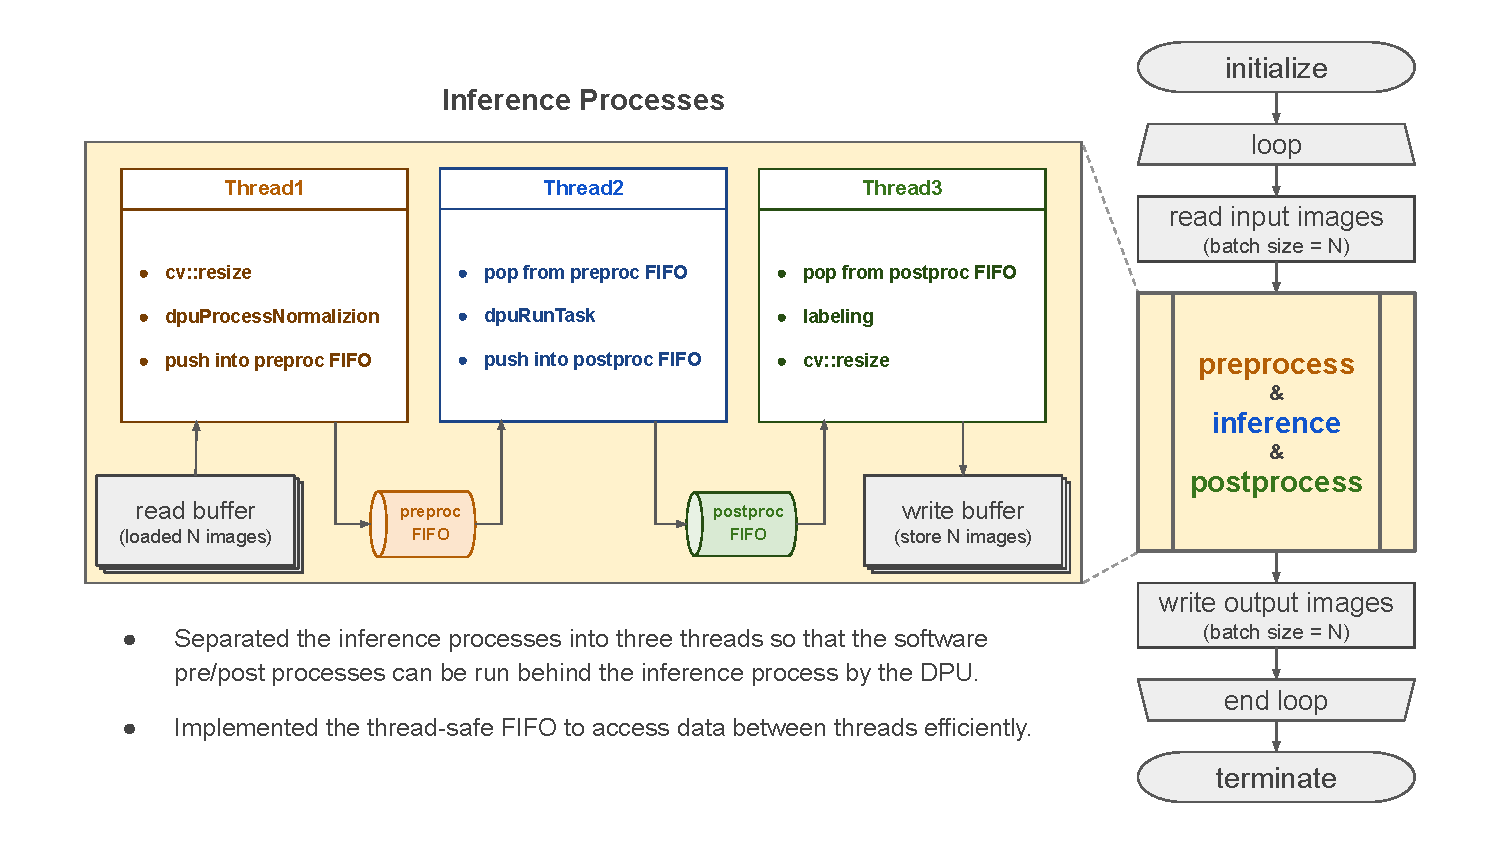
\includegraphics[width=\linewidth]{figures/sw_opt_flowchart_multithread.pdf}
    \caption{マルチスレッド実行時}
    \label{fig:multithread}
  \end{center}
\end{figure}

我々のマルチスレッド実装では,前処理,推論処理,後処理をそれぞれ別スレッド(Thread1, Thread2, Thread3)で実行する.
スレッドセーフなFIFOクラスを実装し,
これを用いてスレッド間でデータを受け渡す実装を行った.
前処理を行うスレッドで処理した入力をDPUによる推論処理を行うスレッドに渡すpreproc FIFOと,
DPUによる推論処理を行うスレッドで得られた出力を後処理を行うスレッドに渡すpostproc FIFOの2つを用いる.
また,マルチスレッド実装では1枚ずつ推論を行うのではなく,複数枚の画像のバッチ処理を行う.
ここでは一度のバッチ処理に使用する入力画像の枚数を $N$ とする.
このような実装により,前処理,推論処理,後処理が擬似的にパイプライン実行され,
実行速度の向上が期待される.

図 \ref{fig:sequence} にマルチスレッド実装の処理のシーケンス図を示す.

\begin{figure}[h]
  \begin{center}
    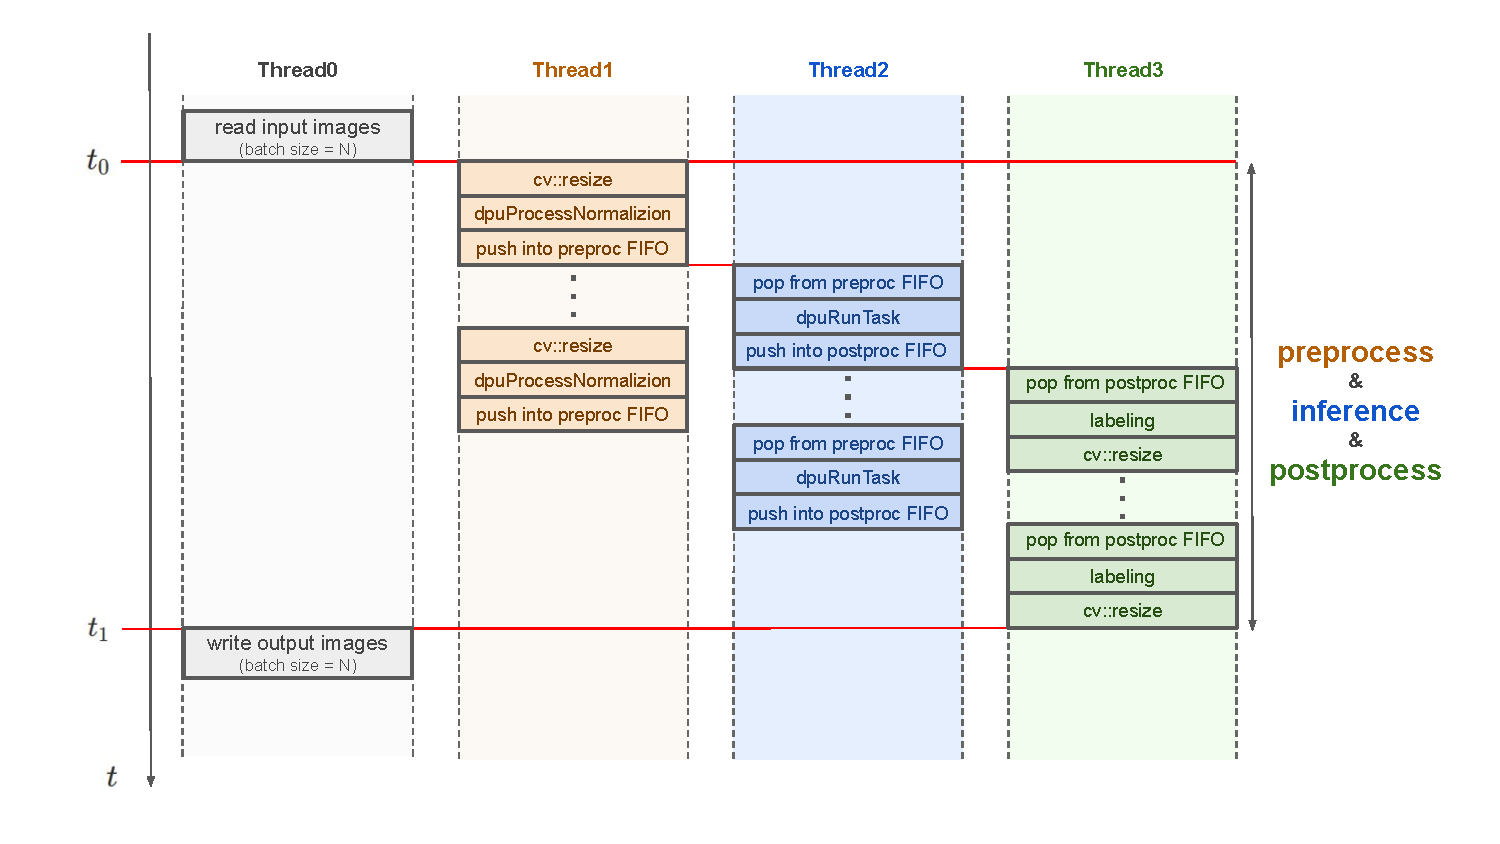
\includegraphics[width=\linewidth]{figures/sw_opt_sequence.pdf}
    \caption{シーケンス図}
    \label{fig:sequence}
  \end{center}
\end{figure}

$N$ 枚の画像をメモリ上に読み込み,推論を行った後に結果をファイル出力するまでの処理のシーケンスを示している.
3つのスレッドが生成される時刻を $t_0$ ,3つのスレッドの全てが終了する時刻を $t_1$ とするとき,
本コンテストにおいて評価対象となる画像1枚あたりの推論処理時間 $t_{\mathrm{inference}}$ は式 \ref{equ:inference} のように計算される.

\begin{equation}
  \label{equ:inference}
  t_{\mathrm{inference}} = \frac{t_1 - t_0}{N}
\end{equation}

ここで,シングルスレッド処理における前処理の縮小の処理時間を $t_{\mathrm{pre\_resize}}$ ,
正規化の処理時間を $t_{\mathrm{pre\_normalize}}$ ,
DPUによる推論の実行時間を $t_{\mathrm{dpu}}$ ,
後処理のラベル付けの処理時間を $t_{\mathrm{post\_labeling}}$ ,
拡大の処理時間を $t_{\mathrm{post\_resize}}$ とする.
また,
preproc FIFOからデータを取得する処理の処理時間を $t_{\mathrm{pop}}$ ,
postproc FIFOにデータを入れる処理の処理時間を $t_{\mathrm{push}}$ とする.
このとき,画像1枚あたりの推論処理時間の予測値 $t_{\mathrm{inference}}^*$ は式 \ref{equ:inference-pred} ように表される.

\begin{equation}
  \label{equ:inference-pred}
    t_{\mathrm{inference}}^* = t_{\mathrm{bottleneck}} + \frac{t_{\mathrm{pre}} + t_{\mathrm{infer}} + t_{\mathrm{post}} - t_{\mathrm{bottleneck}}}{N} + t_\alpha \\
\end{equation}
\begin{equation*}
    \begin{split}
      \text{where} \quad
      t_{\mathrm{bottleneck}}  &= \max \{t_{\mathrm{pre}}, t_{\mathrm{infer}}, t_{\mathrm{post}}\}, \\
      t_{\mathrm{pre}}  &= t_{\mathrm{pre\_resize}} + t_{\mathrm{pre\_normalize}}, \\
      t_{\mathrm{infer}} &= t_{\mathrm{pop}} + t_{\mathrm{dpu}} + t_{\mathrm{push}}, \\
      t_{\mathrm{post}} &= t_{\mathrm{post\_labeling}} + t_{\mathrm{post\_resize}}
    \end{split}
\end{equation*}

ここで, $t_\alpha$ はソフトウェア処理のマルチスレッド化による処理時間のオーバーヘッドを表している.
我々の実装において,画像1枚あたりの推論処理時間は,前処理,DPUによる推論処理,後処理のいずれかの処理時間に律速することが分かる.

次に,前処理,DPUによる推論処理,後処理のそれぞれの具体的な実装を説明する.
ここで示すソースコードは説明のためにいずれも変数名や実装の簡略化等を行っている.
実際のソースコードは後日公開予定のリポジトリ\footnote{https://github.com/Vertical-Beach/ai-edge-contest4}を参照されたい.

\subsubsection{前処理}
前述の通り,前処理では,cv::resizeを用いて入力画像の縮小を行い(Listing \ref{code:preproc}, Line 6),
Vitis-AIのDPUライブラリの関数dpuProcessNormalizionによって各画素値の正規化を行う(Listing \ref{code:preproc}, Line 8-10).

\setcounter{lstnumber}{1}
\begin{lstlisting}[language=c++,firstnumber=last,caption=do\_preprocess(),label=code:preproc]
void do_preprocess() {
  cv::Mat in(in_size, CV_8UC3);
  auto r_buf = read_buffer.begin();
  auto end = false;
  while (!end) {
    cv::resize(*r_buf, in, in.size(), 0, 0, cv::INTER_LINEAR);
    end = (bool)(r_buf == read_buffer.end())
    preproc_fifo.write(ok, end, [&](PreprocFIFOElementType& dst) -> void {
      dpuProcessNormalizion(dst.data(), in.data, in.rows, in.cols, in_mean, in_scale_fix, in.step1());
    });
    r_buf++;
  }
}
\end{lstlisting}

我々が実装したFIFOクラスはread/writeの処理をlambda式で記述するようになっている.
これは,mutexを持つFIFOのバッファを直接参照する記述をクラス定義のスコープ外で行うためである.
このようにすることでFIFO操作の処理を簡潔に記述することが出来る.
FIFOクラスの実装は本レポートの最後に付録として添付している(Listing \ref{code:muitithreadfifo}, Line 16-127).

\subsubsection{DPUによる推論処理}
DPUによる推論処理では,
preproc FIFOからDPUの入力バッファにデータをコピーし(Listing \ref{code:inference}, Line 7),
関数dpuRunTaskの実行による推論後(Listing \ref{code:inference}, Line 9),
DPUの出力バッファからpostproc FIFOに結果をコピーする(Listing \ref{code:inference}, Line 12).

\setcounter{lstnumber}{1}
\begin{lstlisting}[language=c++,firstnumber=last,caption=do\_inference(),label=code:inference]
void do_inference() {
  constexpr auto in_size  = sizeof(int8_t) * IN_IMG_W * IN_IMG_H * IN_IMG_C;
  constexpr auto out_size = sizeof(int8_t) * OUT_IMG_W * OUT_IMG_H * NOF_CLASS;
  auto end = false;
  while (!end) {
    preproc_fifo.read(ok, [&](const PreprocFIFOElementType& src) -> void {
      std::memcpy(in_addr, src.data(), in_size);
    });
    dpuRunTask(task_conv_1);
    end = preproc_fifo.neverReadNextElement();
    postproc_fifo.write(ok, end, [&](PostprocFIFOElementType& dst) -> void {
      std::memcpy(dst.data(), out_addr, out_size);
    });
  }
}
\end{lstlisting}

\subsubsection{後処理}
後処理では,推論結果を参照してラベル画像を生成し(Listing \ref{code:postproc}, Line 6-13),
その後,関数cv::resizeを用いてラベル画像の拡大を行う(Listing \ref{code:postproc}, Line 15).

\setcounter{lstnumber}{1}
\begin{lstlisting}[language=c++,firstnumber=last,caption=do\_postprocess(),label=code:postproc]
void do_postprocess() {
  cv::Mat out(out_size, CV_8UC1);
  auto w_buf = write_buffer.begin();
  while (w_buf != write_buffer.end()) {
    postproc_fifo.read(ok, [&](const PostprocFIFOElementType& dst) -> void {
      auto offset = dst.data();
      for (int ri = 0; ri < out.rows; ri++) {
        for (int ci = 0; ci < out.cols; ci++) {
          const auto max_itr = std::max_element(offset, offset + NOF_CLASS);
          out.at<uint8_t>(ri, ci) = (uint8_t)(std::distance(offset, max_itr));
          offset += NOF_CLASS;
        }
      }
    });
    cv::resize(out, *w_buf, (*w_buf).size(), 0, 0, cv::INTER_NEAREST);
    w_buf++;
  }
  if (!postproc_fifo.neverReadNextElement()) {
    throw std::runtime_error("[ERROR] The data is still in the postproc FIFO.");
  }
}
\end{lstlisting}

ここで,本推論アプリケーションの最終的な出力となる 1216*1936 のラベル画像は,
各ピクセルに0から5の値が格納されたグレイスケール画像であることに注意されたい.
この0から5の値は順に「乗用車」,「歩行者」,「信号」,「車道・駐車場」,「その他」に相当する.
